\newpage
\subsection{Propagating coastal surface signal in an \OGCM{}: Australia's East Coast}
\label{S:plan_CTW}

\subsubsection{Problem and motivation}
Coastally trapped waves (CTW) are a phenomena of special interest to operational sea level forecasting in Australia. \\
Anecdotally, \BL{} represents propagating coastal sea level signals which in principle can provide a valuable addition to forecast guidance used within the \BOM.  The extent to which freely propagating CTWs are skilfully forecast and why is not well understood - especially with regard to the extension of the coastal wave guide around Australia's East coast.\\



Powerful surface-apparent CTWs are characteristic of the Southern Coast of Australia and commonly propagate eastward at similar rates to the forcing weather system \citep{Taylor:2009vw}.\\
For this study, regional focus is restricted to the \emph{East Coast} for the following reasons:
\begin{inparaenum}[(a)]
\item extensive discussion of East Coast CTWs in the scientific literature (though typically focussed on subsurface currents);
\item well spaced coastal tide gauge array;
\item indications the \BL{} skill degrades towards the North and within the GBR;  
\item expectation that freely propagating modes may be identifiable in this region;
\item operational impact due to population density.
%\item opportunity to utilise the \ER{} model.
\end{inparaenum}


\subsubsection{Data sources}
Sea level anomaly has been compiled from operational \BL{} analyses during the Austral winter of 2012, a period with no system changes.\\  
Tide gauge data available for this region offers a uniquely dense and well-spaced coastal array - in contrast to other parts of Australia.   The instruments available for this study are operated by the Bureau of Meteorology, Manly Hydraulics Laboratory and the Queensland Department of Environment and Heritage Protection.  Locations included are indicated in Figure \ref{fig:tide_gauges}.\\

\begin{figure}[!h]
	\centering
	\subfloat[tide gauges] {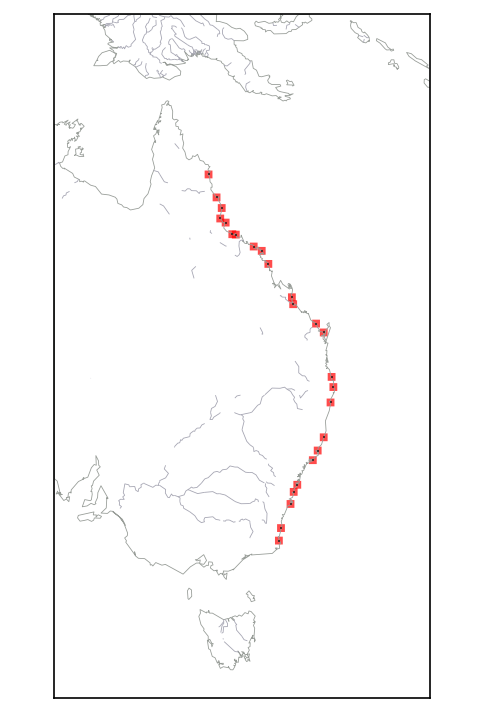
\includegraphics[width=40mm]{figures_3/plot_locations_Australia.png}}
	\subfloat[Illustration of spatial HEOF modes derived from observation array]  {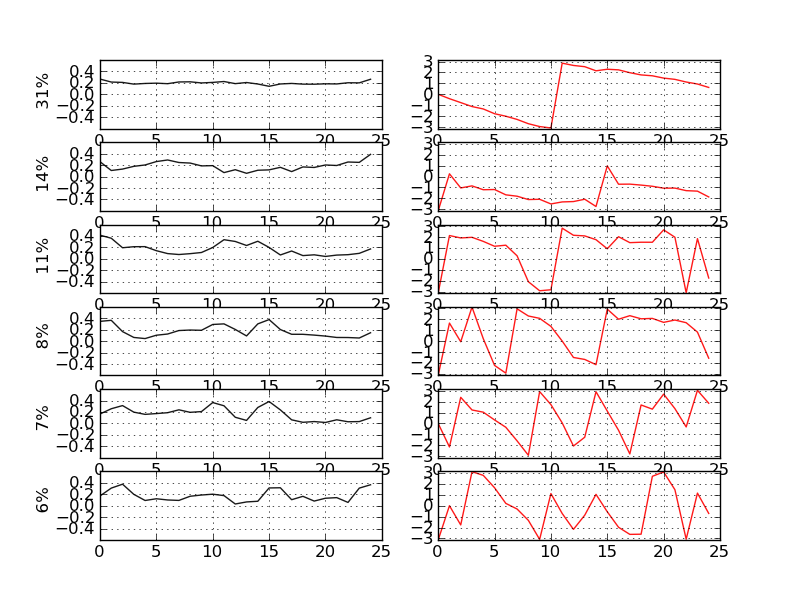
\includegraphics[width=80mm]{figures_3/HEOF_modes_obs.png}}\\
	%\subfloat[Approximate along-shore distance]  {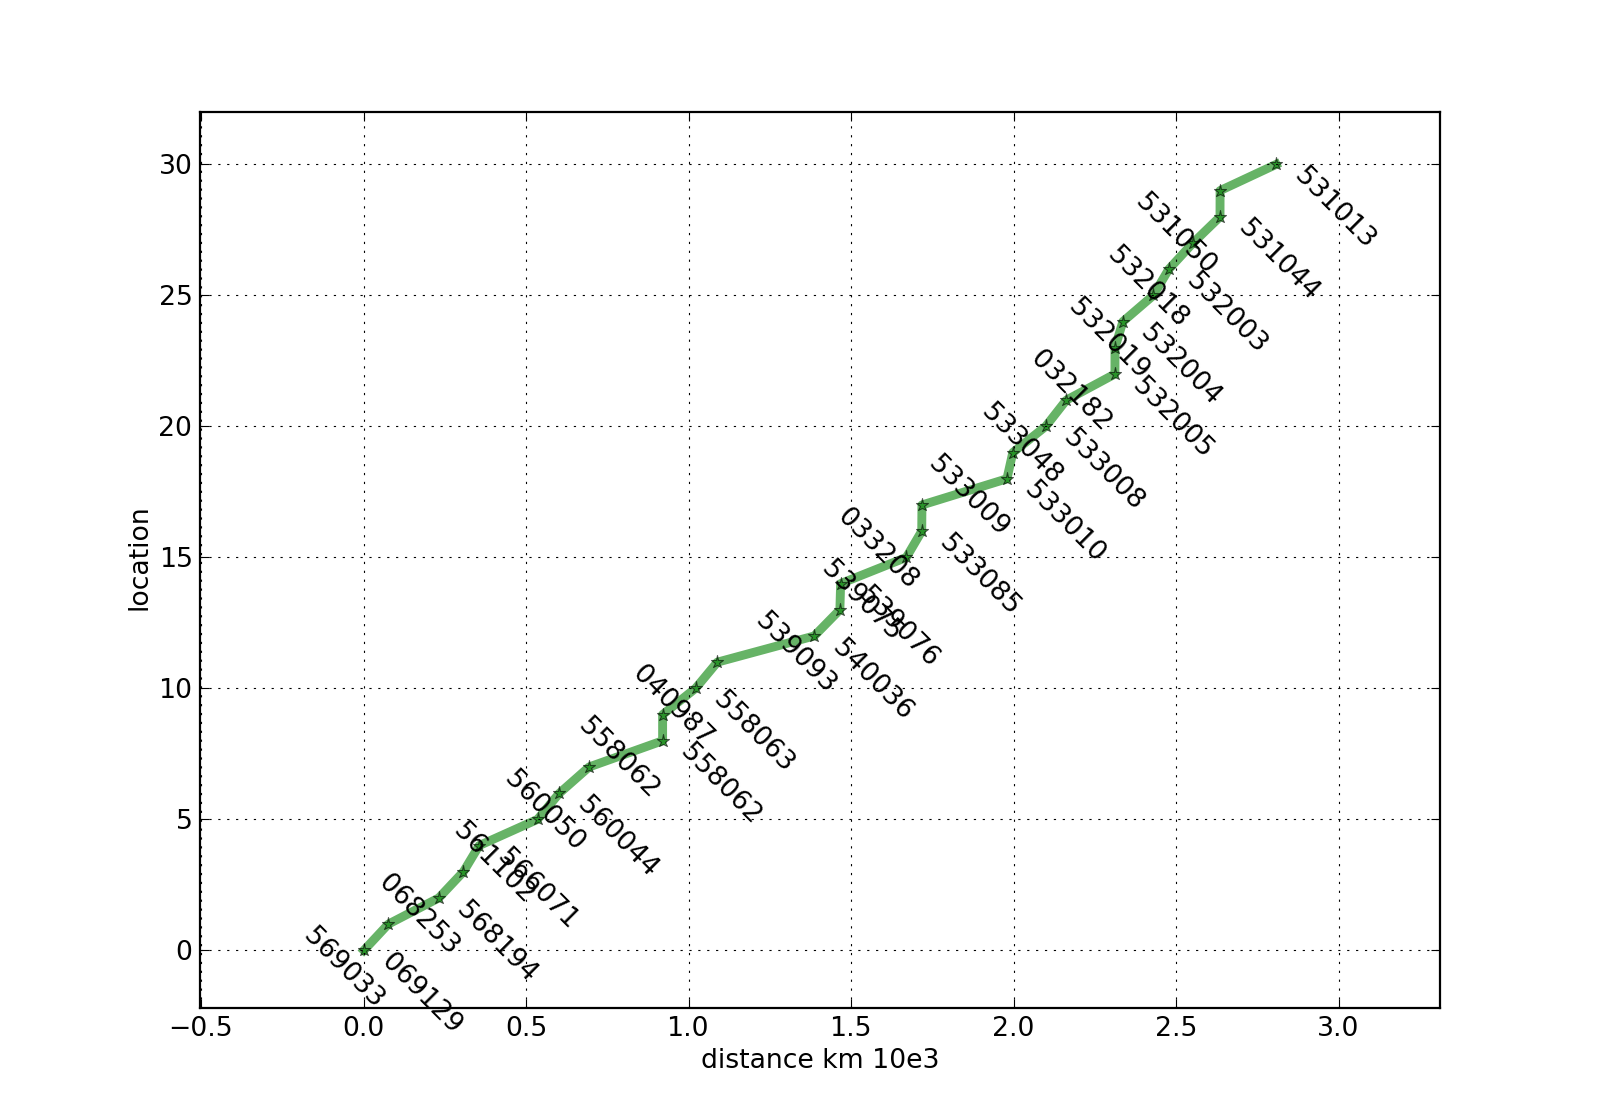
\includegraphics[width=120mm]{figures_3/plot_station_distance.png}}\\
	\caption{Observation locations}
	\label{fig:tide_gauges}
\end{figure}

Depending on availability, simulations from higher resolution ocean models produced by the \BOM{} may be accessed and used for cross-comparison.


\subsubsection{Method outlook}
In essence this study involves the diagnosis of model performance using observations.  Aspects related to coastal propagation are the primary focus.\\ 
Comparison is not physically meaningful without substantial pre-processing.  In the first instance, the observations will be reduced to a SLA quantity by de-tiding.  Subsequently, a signal decomposition method will be employed in order isolate, quantify and diagnose aspects of coastal propagation.  A Hilbert Empirical Orthogonal Functions (HEOF) technique appears to offer an appropriate perspective in this regard.  Previous discussion of related methods offer some insight [REFS]\\

% steps
Work steps sketch:
\begin{enumerate}
\item Prepare observational dataset - including download of additional quality controlled data from MHL and application of appropriate de-tiding; 
\item Characterise observations by spectral content with regard to spacing along coast;
\item Identify candidate propagation events;
\item Characterise raw model forecast skill at each location;
\item Explore the application of HEOF analysis to data subset: Can HEOF modes identify propagation? Does the decomposition offer any insight into model/obs comparison?
\end{enumerate}




This study aims to understand the specific characteristics and limitations of \BL{} along the East Coast; in light of the literature addressing CTWs.   Ultimately, the results may inform the provision of forecasts and prospective system modifications.



%Questions to be addressed:
%\begin{itemize}
%\item where does \BL{} offer any forecast skill on the East Coast?
%\item can the nature of forecast errors be diagnosed?
%\item can error diagnosis guide forecast interpretation and/or suggest system improvements?
%\end{itemize}



%\item Asses \NWP{} forcing:
%%\subitem Regrid $\tau$ from \AG{} and \AR{} the same \OFAM{} target grid.
%\subitem Any systematic biases in \AG{}?

%\item Decompose $\eta_t(t,lat,lon)$ into approximate categories of locally and remotely forced.  
%\subitem Assess decomposed $eta_t$ skill against observations. 
%\subitem Is the relative impact of local versus remote forcing identifyable?

%\item Compare \BL{} against \ER{} $\eta_t$ for the GBR region. 
%\subitem Is raw skill of \ER{} better than \BL{}?
%\subitem Diagnose difference in \ER{}.  
%\end{enumerate}

%\begin{figure}[!h]%
%	\centering
	%\subfloat[overlaid timeseries of observations and eta] {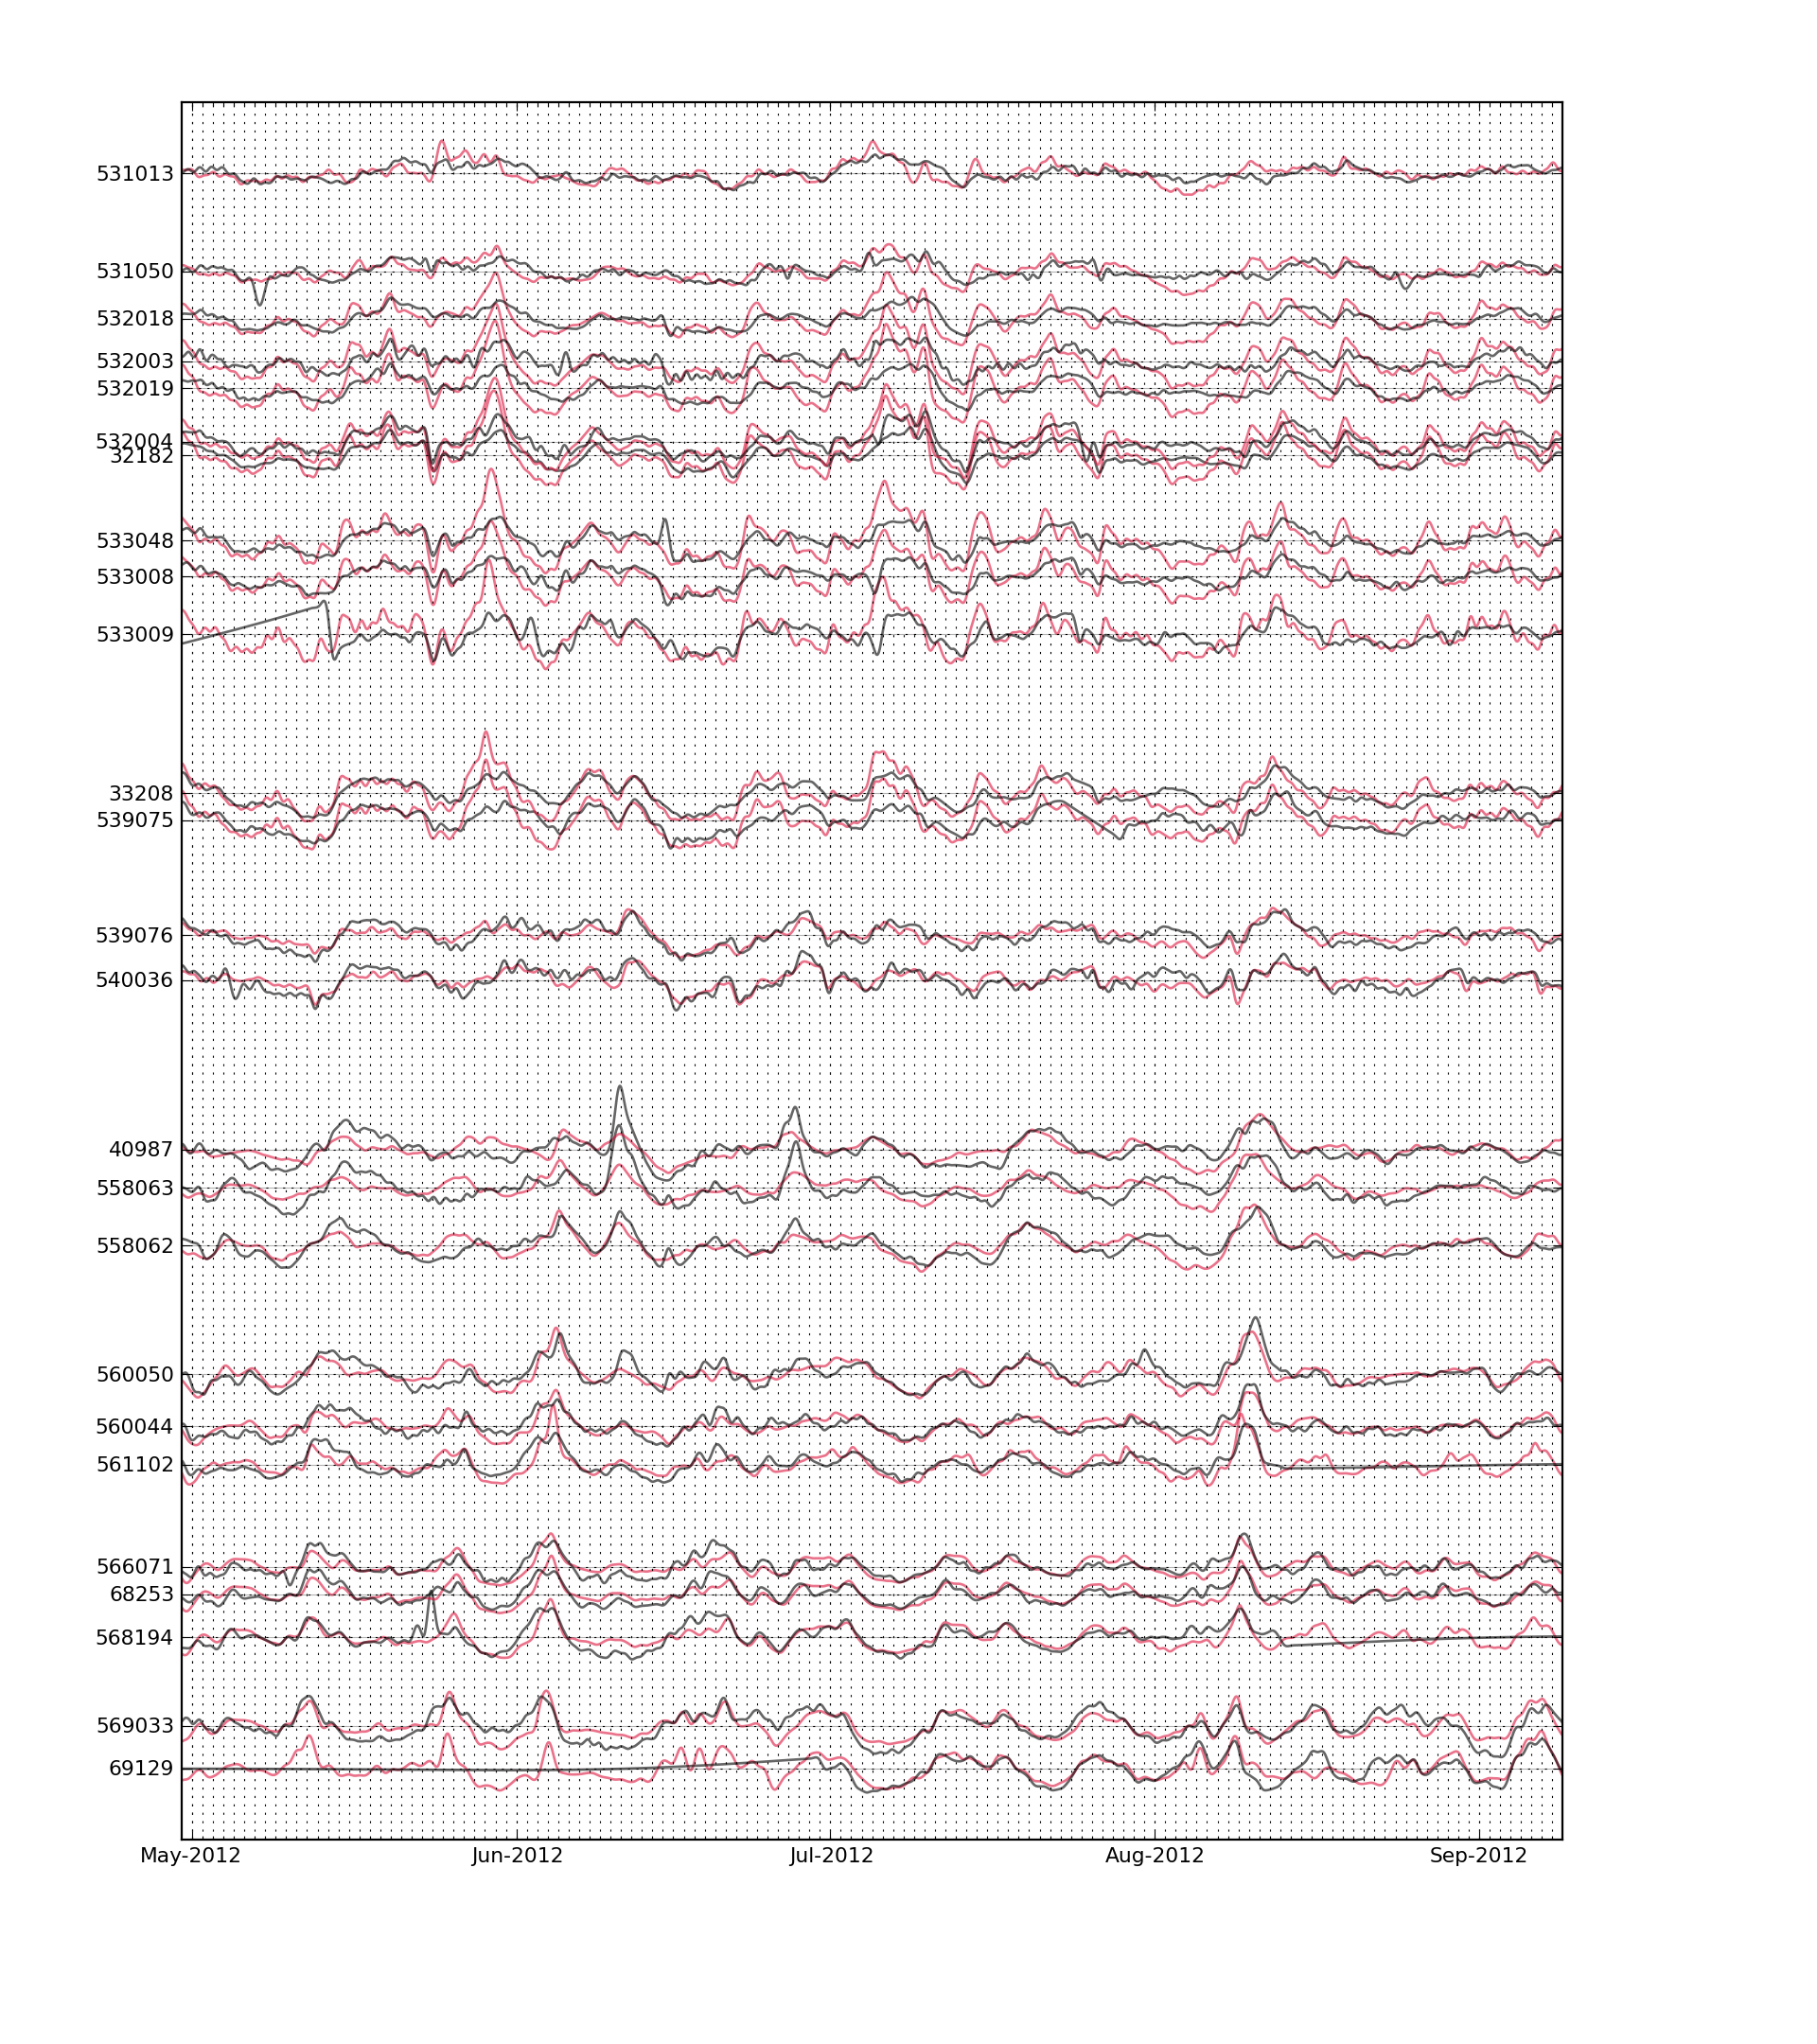
\includegraphics[width=100mm]{figures_3/plot_tsstack_bpass60p0_1p2.png}}\\
%	\subfloat[illustration of spatial HEOF modes derived from observation array]  {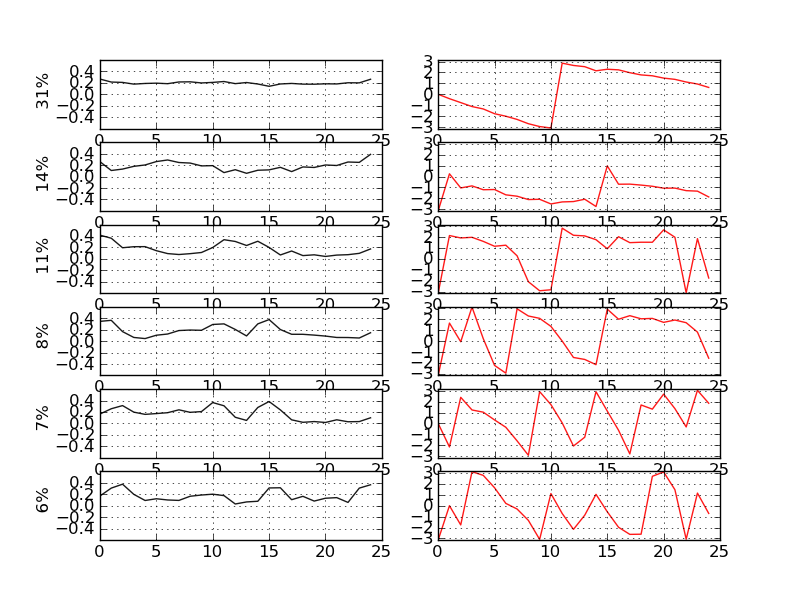
\includegraphics[width=120mm]{figures_3/HEOF_modes_obs.png}}\\
%	\caption{Observation locations}
%	\label{fig:HEOF_overview}
%\end{figure}


